% Created 2016-08-29 Mon 15:38
\documentclass[11pt]{article}
\usepackage[utf8]{inputenc}
\usepackage[T1]{fontenc}
\usepackage{fixltx2e}
\usepackage{graphicx}
\usepackage{grffile}
\usepackage{longtable}
\usepackage{wrapfig}
\usepackage{rotating}
\usepackage[normalem]{ulem}
\usepackage{amsmath}
\usepackage{textcomp}
\usepackage{amssymb}
\usepackage{capt-of}
\usepackage{hyperref}
\usepackage{minted}
\author{章立}
\date{\today}
\title{}
\hypersetup{
 pdfauthor={章立},
 pdftitle={},
 pdfkeywords={},
 pdfsubject={},
 pdfcreator={Emacs 24.5.1 (Org mode 8.3.4)}, 
 pdflang={English}}
\begin{document}

\tableofcontents

\section{This Week}
\label{sec:orgheadline17}
\subsection{\href{https://github.com/BVLC/caffe/tree/85bb397acfd383a676c125c75d877642d6b39ff6/examples/feature_extraction}{extract feature}}
\label{sec:orgheadline6}
\subsubsection{using caffe to extract features}
\label{sec:orgheadline1}
\begin{minted}[]{sh}
find `pwd`/examples/images -type f -exec echo {} \; > examples/_temp/temp.txt
sed "s/$/ 0/" examples/_temp/temp.txt > examples/_temp/file_list.txt
cd $CAFFE
./build/tools/extract_features models/bvlc_reference_caffenet/bvlc_reference examples/_temp/imagenet_val.prototxt example/_temp/feature fc7 10 lmdb GPU 0
\end{minted}
\subsubsection{general command for extract feature using caffe}
\label{sec:orgheadline2}
\begin{minted}[]{sh}
extract_features pretrained_net_param  feature_extraction_proto_file \
extract_feature_blob_name1[,name2,...]  save_feature_dataset_name1[,name2,...] \
num_mini_batches  db_type  [CPU/GPU] [DEVICE_ID=0]
\end{minted}
\begin{itemize}
\item 参数1是模型参数(.caffemodel)文件的路径。

\item 参数2是描述网络结构的prototxt文件。程序会从参数1的caffemodel文件里找对应名称的layer读取参数。

\item 参数3是需要提取的blob名称,对应网络结构prototxt里的名称。blob名称可以
\end{itemize}
有多个,用逗号分隔。每个blob提取出的特征会分开保存。

\begin{itemize}
\item 参数4是保存提取出来的特征的数据库路径,可以有多个,和参数3中一一对应,
\end{itemize}
以逗号分隔。如果用LMDB的话,路径必须是不存在的(已经存在的话要改名或者
删除)。 

\begin{itemize}
\item 参数5是提取特征所需要执行的batch数量。这个数值和prototxt里DataLayer中
\end{itemize}
的Caffe的DataLayer(或者ImageDataLayer)中的batch\(_{\text{size参数相乘}}\),就是会被
输入网络的总样本数。设置参数时需要确保batch\(_{\text{size}}\) * num\(_{\text{mini}}_{\text{batches等}}\)
于需要提取特征的样本总数,否则提取的特征就会不够数或者是多了。 

\begin{itemize}
\item 参数6是保存特征使用的数据库类型,支持lmdb和leveldb两种(小写)。推荐使用
\end{itemize}
lmdb,因为lmdb的访问速度更快,还支持多进程同时读取。 

\begin{itemize}
\item 参数7决定使用GPU还是CPU,直接写对应的三个大写字母就行。省略不写的话默
\end{itemize}
认是CPU。 

\begin{itemize}
\item 参数8决定使用哪个GPU,在多GPU的机器上跑的时候需要指定。省略不写的话默
\end{itemize}
认使用0号GPU。 

注意事项
\begin{itemize}
\item 提取特征时,网络运行在Test模式下
\begin{itemize}
\item Dropout层在Test模式下不起作用,不必担心dropout影响结果
\item Train和Test的参数写在同一个Prototxt里的时候,改参数的时候注意不
要改错地方(比如有两个DataLayer的情况下)
\end{itemize}
\item 减去均值图像
\begin{itemize}
\item 提取特征时,输入的图像要减去均值
\item 应该减去训练数据集的均值
\end{itemize}
\item 提取哪一层
\begin{itemize}
\item 不要提取Softmax网络的最后一层(如AlexNet的fc8),因为最后一层已经
是分类任务的输出,作为特征的可推广性不够好
\end{itemize}
\end{itemize}
\subsubsection{read from lmdb}
\label{sec:orgheadline3}
\begin{minted}[]{python}
import numpy as np
import caffe
import lmdb
from caffe.proto import caffe_pb2

fea_lmdb = lmdb.open('featureA')
lmdb_txn = fea_lmdb.begin()
lmdb_cursor = txn.cursor()
features = []

for key, value in lmdb_cursor:
    datum = caffe_pb2.Datum()
    datum.ParseFromString(value)
    data = caffe.io.datum_to_array(datum)
    features.append(data)
\end{minted}
\subsubsection{image recognition using \texttt{cos} similarity measure}
\label{sec:orgheadline4}
\begin{minted}[]{python}
import numpy as np
import caffe
import lmdb
from caffe.proto import caffe_pb2
from scipy import spatial


# 3 steps to read form lmdb
fea_lmdb = lmdb.open('/root/caffe/examples/_temp/featureA')
lmdb_txn = fea_lmdb.begin()
lmdb_cursor = lmdb_txn.cursor()
features = []

for key, value in lmdb_cursor:
    datum = caffe_pb2.Datum()
    # Parse from serialized data
    datum.ParseFromString(value)
    data = caffe.io.datum_to_array(datum)
    features.append(data)

out = []
for f in features:
    out.append(f.flatten())

n = len(out)
similarity = np.zeros((n, n), dtype=np.double)

for i in xrange(n):
    for j in xrange(n):
      # cosin distance
        similarity[i, j] = 1 - spatial.distance.cosine(out[i], out[j])
\end{minted}
\subsubsection{\texttt{cos} similarity result}
\label{sec:orgheadline5}
\begin{itemize}
\item accuracy (true ture) : 53 / 55
\end{itemize}
\begin{minted}[]{python}
a = similarity[0:10, 0:10]
  array([[ 1.        ,  0.63231419,  0.84345085,  0.73587363,  0.58211244,
           0.67306891,  0.46881317,  0.56938226,  0.65432654,  0.55240935],
         [ 0.63231419,  1.        ,  0.68508232,  0.56741804,  0.74116358,
           0.81706845,  0.71951714,  0.75391089,  0.78529276,  0.74174079],
         [ 0.84345085,  0.68508232,  1.        ,  0.78416825,  0.61635946,
           0.72695667,  0.54473343,  0.60050371,  0.70046374,  0.58715887],
         [ 0.73587363,  0.56741804,  0.78416825,  1.        ,  0.50801387,
           0.60814318,  0.5046651 ,  0.52948304,  0.68054069,  0.49502061],
         [ 0.58211244,  0.74116358,  0.61635946,  0.50801387,  1.        ,
           0.88589477,  0.56183335,  0.72687896,  0.60917844,  0.87135289],
         [ 0.67306891,  0.81706845,  0.72695667,  0.60814318,  0.88589477,
           1.        ,  0.63597132,  0.76000156,  0.7042399 ,  0.87401555],
         [ 0.46881317,  0.71951714,  0.54473343,  0.5046651 ,  0.56183335,
           0.63597132,  1.        ,  0.58212342,  0.64319046,  0.6254508 ],
         [ 0.56938226,  0.75391089,  0.60050371,  0.52948304,  0.72687896,
           0.76000156,  0.58212342,  1.        ,  0.74652927,  0.72233884],
         [ 0.65432654,  0.78529276,  0.70046374,  0.68054069,  0.60917844,
           0.7042399 ,  0.64319046,  0.74652927,  1.        ,  0.61672591],
         [ 0.55240935,  0.74174079,  0.58715887,  0.49502061,  0.87135289,
           0.87401555,  0.6254508 ,  0.72233884,  0.61672591,  1.        ]])

np.sum(a > 0.5)
96
\end{minted}
\begin{itemize}
\item false true : 2 / 100
\end{itemize}
\begin{minted}[]{python}
In [1]: ab = similarity[0:10, 10:]

In [2]: ab
Out[2]:
array([[ 0.2842583 ,  0.37596221,  0.27628312,  0.12041221,  0.29636999,
         0.13618284,  0.1381707 ,  0.17832465,  0.21937008,  0.40752771],
       [ 0.32961919,  0.49064045,  0.29595205,  0.093565  ,  0.39657901,
         0.17370467,  0.15514055,  0.2672414 ,  0.31652746,  0.46922921],
       [ 0.31926577,  0.45413662,  0.26234978,  0.1560283 ,  0.30816957,
         0.15273065,  0.16850629,  0.22604249,  0.25764858,  0.44164225],
       [ 0.26623039,  0.3611369 ,  0.20121232,  0.11351721,  0.21726182,
         0.11916629,  0.1431136 ,  0.20710409,  0.22387793,  0.31652456],
       [ 0.30927462,  0.35910132,  0.2650208 ,  0.08663475,  0.37263798,
         0.10722143,  0.09815253,  0.17950735,  0.20988739,  0.50689106],
       [ 0.32089366,  0.40492257,  0.28595893,  0.09466663,  0.37709065,
         0.10737807,  0.10595637,  0.19340299,  0.23139416,  0.51704389],
       [ 0.29795872,  0.3890121 ,  0.26349005,  0.08589599,  0.36945176,
         0.16923292,  0.11844475,  0.24970864,  0.31689723,  0.36337912],
       [ 0.28911623,  0.33516171,  0.30897566,  0.12046317,  0.36436887,
         0.10022814,  0.14957088,  0.29092572,  0.3343103 ,  0.47673998],
       [ 0.31926479,  0.43550698,  0.31588098,  0.09185497,  0.33737191,
         0.15741605,  0.16819127,  0.34134218,  0.38785466,  0.41883917],
       [ 0.29190126,  0.3130953 ,  0.25801771,  0.07097081,  0.34608239,
         0.09577894,  0.0842366 ,  0.14185045,  0.19112799,  0.47368384]])

In [3]: np.sum(ab > 0.5)
Out[3]: 2
\end{minted}

\subsection{Cuda Note}
\label{sec:orgheadline16}
\subsubsection{Configuring the kernel launch}
\label{sec:orgheadline7}
\texttt{kernel<<<grid of block, block of threads>>>(...)}

\texttt{square<<<dim3(bx,by,bz), dime(tx,ty,tz), sharem>>>(...)}

\begin{itemize}
\item grid of blocks : bx * by * bz
\item block of threads : tx * ty * tz
\item shared memory per block in bytes
\end{itemize}
\subsubsection{Convert color to black and white}
\label{sec:orgheadline8}
\[I = (R + G + B) / 3\]
\[I = .299f * R + .587f * G + .114f * B\]
\subsubsection{\href{http://docs.nvidia.com/cuda/cuda-compiler-driver-nvcc/index.html#cuda-programming-model}{ \texttt{nvcc} introduction}}
\label{sec:orgheadline9}
\subsubsection{cs344 Note}
\label{sec:orgheadline10}
\begin{itemize}
\item GPU is responsible for allocating blocks to SM(streaming multiprocessors)
\item A block cannot run on more than one SM
\item An SM may run more than one block
\item All the SMs are running in parallel
\item Threads in different block shouldn't cooperate
\item Cuda make few guarantees about when and where thread blocks will run
\item consequences
\begin{itemize}
\item no assumptions blocks -> SM
\item no communication between blocks
\end{itemize}
\item CUDA guarantees that:
\begin{itemize}
\item all threads in a block run on the same SM at the same time
\item all blocks in a kernel finish before any blocks from next run
\end{itemize}
\item threadIdx : thread within block threadIdx.x threadIdx.y
\begin{itemize}
\item blockDim : size of block
\item blockIdx : block within grid
\item gridDim : size of grid
\end{itemize}
\end{itemize}
\subsubsection{GPU memory model}
\label{sec:orgheadline11}
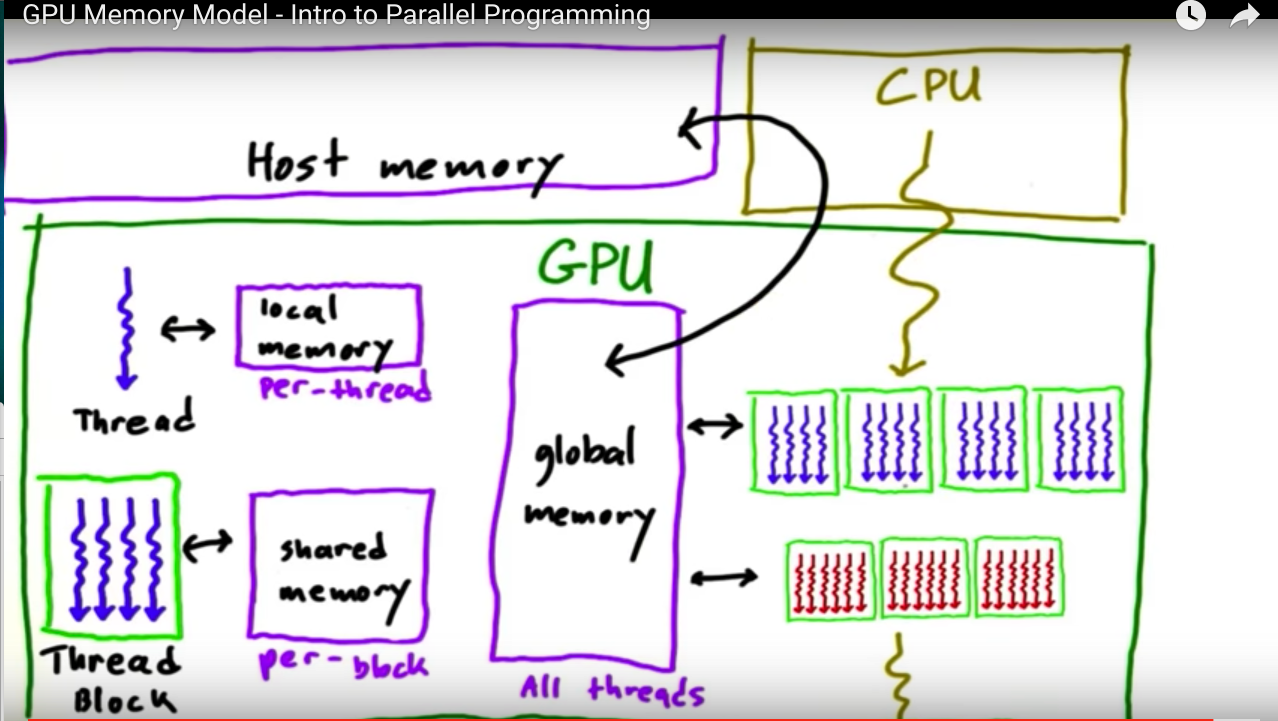
\includegraphics[width=.9\linewidth]{./images/gpu-memory-model.png}
\begin{itemize}
\item All threads from a block can access the same variable in that
block shared memory
\item Threads from two different blocks can access the same variable in
global memory
\item Threads from different blocks have their own copy of local
variables in local memory
\item Threads from the same block have their own copy of local variables
in local memory
\end{itemize}

\subsubsection{barrier}
\label{sec:orgheadline12}
point in program where threads stop and wait. when all threads have
reached the barrier, they can proceed.
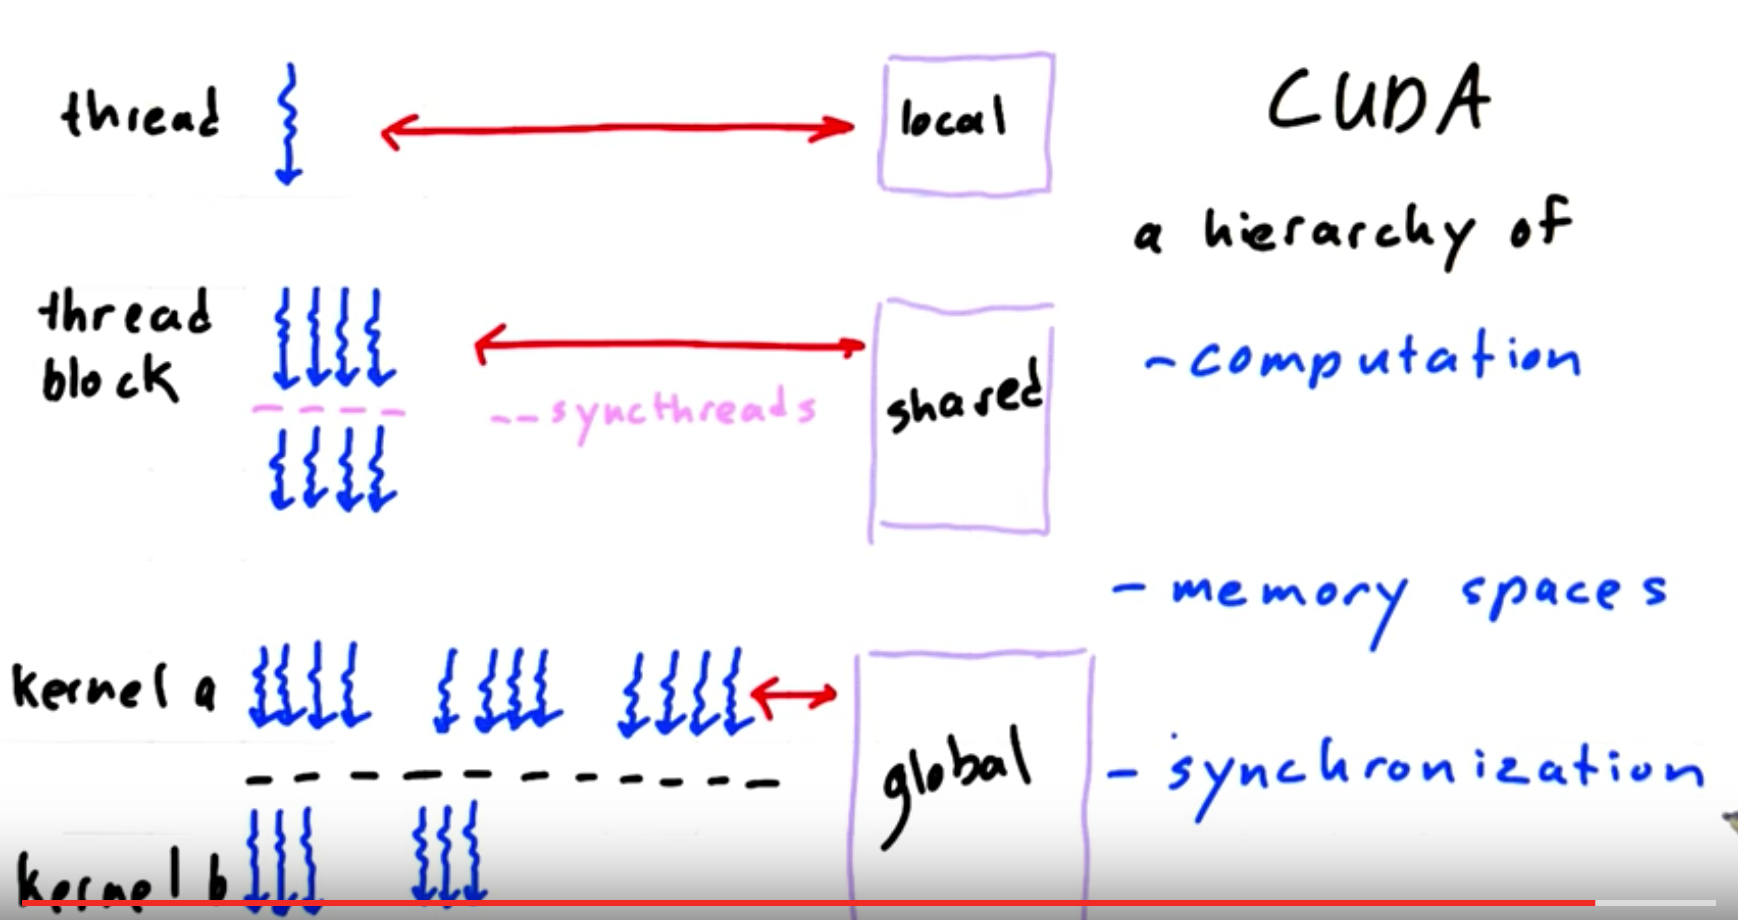
\includegraphics[width=.9\linewidth]{./images/synchronized.png}
\subsubsection{High-level strategies}
\label{sec:orgheadline13}
\begin{enumerate}
\item Maximize arithmetic intensity
\end{enumerate}
\[\frac{Math}{Memory}\]
\begin{itemize}
\item maximize compute ops per thread
\item minimize time spent on memory per thread
\begin{itemize}
\item move frequently-accessed data to fast memory
local > shared >> global >> cpu memory
\end{itemize}
\end{itemize}
coalesce memeory
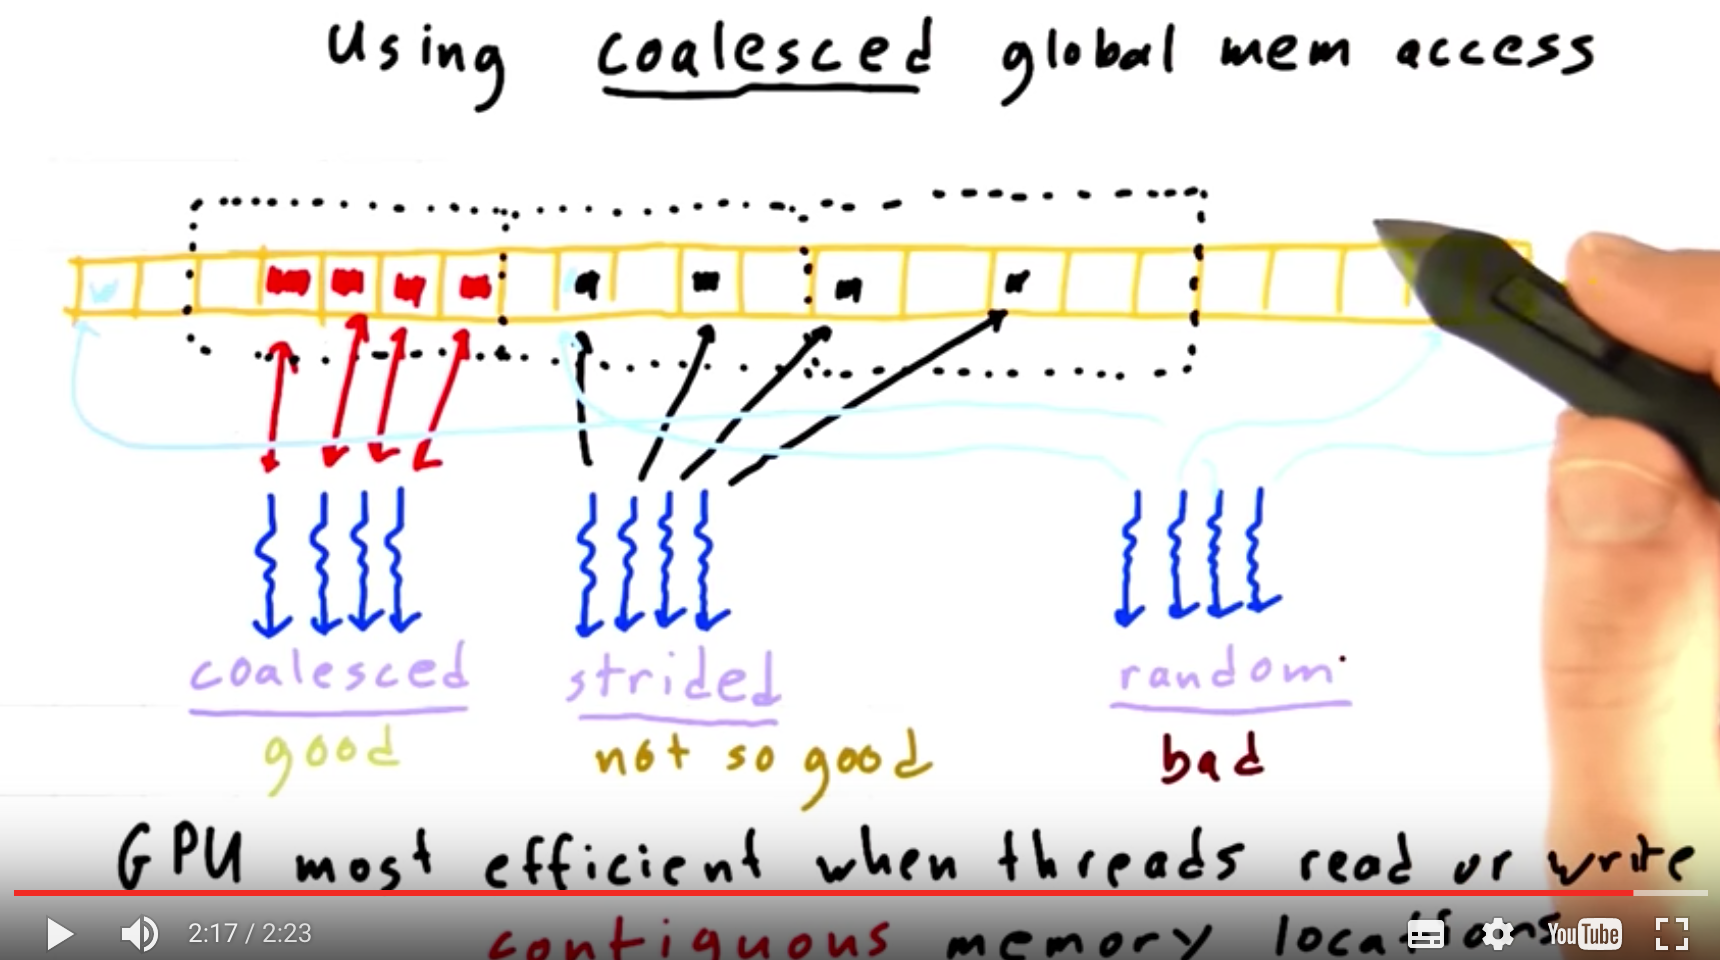
\includegraphics[width=.9\linewidth]{./images/coalesce.png}
\begin{enumerate}
\item avoid thread divergence
\end{enumerate}

\subsubsection{\texttt{cudaMalloc}}
\label{sec:orgheadline14}
\begin{minted}[]{c++}
float *device_data=NULL;  
size_t size = 1024*sizeof(float);  
cudaMalloc((void**)&device_data, size);
\end{minted}
而 \texttt{device\_data} 这个指针是存储在主存上的。之所以取 \texttt{device\_data} 的地
址,是为了将 \texttt{cudaMalloc} 在显存上获得的数组首地址赋值给 \texttt{device\_data}
。在函数中为形参赋值是不会在实参中繁盛变化的,但是指针传递的是地址 

\subsubsection{{\bfseries\sffamily TODO} \href{file:///Users/zhangli/Documents/Library.papers3/Files/1E/1ED49076-5D40-4E5F-B232-918B17EA1596.pdf}{What Every Programmer Should Know About Memory}}
\label{sec:orgheadline15}

\section{Next Week}
\label{sec:orgheadline20}
\subsection{Cuda programming}
\label{sec:orgheadline18}
\subsection{caffe}
\label{sec:orgheadline19}
\end{document}
